\section{Introduction}
Benchmarking and profiling are fundamental processes for evaluating the computational performance and reliability of \acrshort{pra} tools. These processes enable the identification of performance bottlenecks, inform optimization strategies, and provide a basis for fair comparison between different quantification engines. This chapter presents a systematic benchmarking and profiling study of two PRA quantification engines: scram and SAPHSOLVE. The study uses a combination of synthetic models, the Aralia dataset, and generic Pressurized Water Reactor (PWR) models. The benchmarking methodology, performance metrics, and key findings are presented, followed by a detailed discussion of profiling results and their implications for future tool development.

\section{Benchmarking Methodology}
The benchmarking and profiling framework adopted in this study is inspired by a diagnostic methodology analogous to medical diagnostics. Just as a physician conducts an initial assessment followed by more detailed investigations, the evaluation of PRA tools begins with quick diagnostics through benchmarking, followed by detailed diagnostics via profiling. The overall workflow is illustrated in Figure~\ref{fig:diagnostic}, which serves as an overview of the approach.

\begin{figure}[h!]
    \centering
    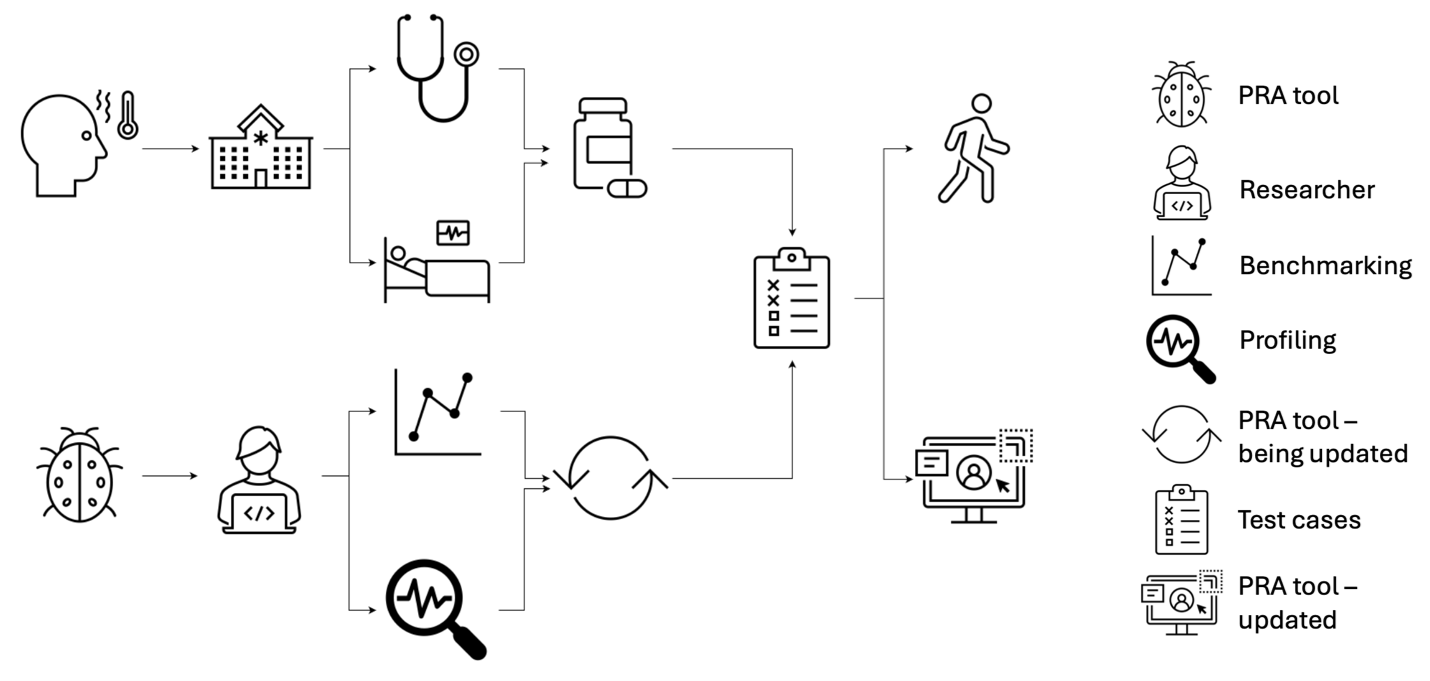
\includegraphics[width=0.9\textwidth]{3_identifying_gaps/benchmarking/profiling_methods/figures/diagnostic.png}
    \caption{Overview of diagnostic methodology for a PRA tool.}
    \label{fig:diagnostic}
\end{figure}

The benchmarking phase focuses on measuring key performance metrics such as CPU time and memory usage. However, benchmarking alone is insufficient for uncovering the root causes of inefficiency. Profiling is therefore employed to analyze the internal behavior of the code, identify computational hotspots, and guide targeted improvements. The combined outcomes of benchmarking and profiling inform an enhancement roadmap, which may include code optimization and the adoption of parallel computing strategies.

\subsection{Benchmarking Process}
The benchmarking process is structured around three essential components: the PRA model, the quantification tool, and the benchmarking configuration. Figure~\ref{fig:benchmarking_methodology} provides a schematic representation of the benchmarking methodology.

\begin{figure}[h!]
    \centering
    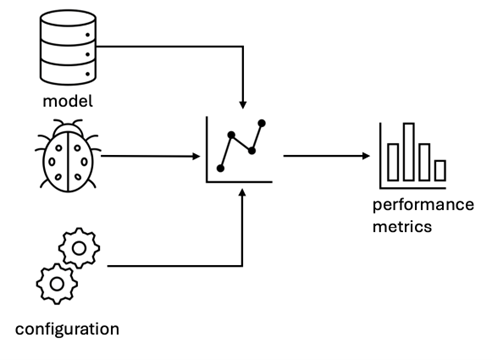
\includegraphics[width=0.5\textwidth]{3_identifying_gaps/benchmarking/profiling_methods/figures/benchmarking_methodology.png}
    \caption{Benchmarking methodology for a PRA tool.}
    \label{fig:benchmarking_methodology}
\end{figure}

Synthetic models are generated to facilitate controlled and reproducible comparisons between quantification engines. The model generator is parameterized to produce fault trees with varying numbers of basic events, gate types, and common-cause failures. Table~\ref{tab:model_generator_parameters} summarizes the key arguments and configurations used in the case study.

\begin{table}[htbp]
    \centering
    \caption{PRA model generator arguments with case study configurations.}
    \label{tab:model_generator_parameters}
    \begin{tabular}{|c|l|l|l|}
        \hline
        \textbf{Argument} & \textbf{Description} & \textbf{Option} & \textbf{Configuration} \\
        \hline
        1 & Name for fault tree & \texttt{--ft-name} & Autogenerated \\
        2 & Name for the root gate & \texttt{--root} & Root \\
        3 & Seed for PRNG & \texttt{--seed} & 123 \\
        4 & Number of basic events & \texttt{--num-basic} & 100:50:5000 \\
        5 & Average number of gate arguments & \texttt{-num-args} & 3.0 \\
        6 & Weights for gates [AND, OR, K/N, NOT, XOR] & \texttt{--weights-g} & [1,1,1,0,0] \\
        7 & Avg. \% of common basic events per gate & \texttt{--common-b} & 0.3 \\
        8 & Avg. \% of common gates per gate & \texttt{--common-g} & 0.1 \\
        9 & Avg. number of parents for common basic events & \texttt{--parents-b} & 2 \\
        10 & Avg. number of parents for common gates & \texttt{--parents-g} & 2 \\
        11 & Number of gates & \texttt{-g} or \texttt{-num-gate} & 0 \\
        12 & Maximum probability of basic events & \texttt{---max-prob} & 0.05 \\
        13 & Minimum probability of basic events & \texttt{--min-prob} & 0.01 \\
        14 & Number of house events & \texttt{--num-house} & 0 \\
        15 & Number of common-cause-failure groups & \texttt{--num-ccf} & 0 \\
        16 & Output file for the fault tree & \texttt{-o} or \texttt{-out} & XML or JSInp \\
        17 & Apply the other format to the output & \texttt{--other} & --saphsolve \\
        \hline
    \end{tabular}
\end{table}

The number of basic events is systematically varied from 100 to 5,000 in increments of 50, resulting in 99 distinct models for each engine. Gate types are randomly assigned, with AND, OR, and K/N gates occurring with equal probability. Notably, scram accepts truncation parameters via the command line, while SAPHSOLVE requires them in the input file. A probability truncation value of $10^{-20}$ is used, and no size truncation is applied. Common-cause failures, uncertainty analysis, and importance measures are excluded from this study.

The benchmarking environment is standardized to ensure fair comparison. All tools are executed with a 30-minute wall-clock time limit, 16 GB RAM, and a single CPU core. BenchExec is used to manage resource allocation and collect performance data.

\subsection{Profiling Process}
Profiling is conducted to gain deeper insight into the internal performance characteristics of the quantification engines. The profiling methodology is depicted in Figure~\ref{fig:profiling}. A challenging PRA model is selected based on benchmarking results to ensure sufficient runtime for meaningful analysis. The quantification engine is compiled in release mode with maximum optimization and debug information enabled. Intel VTune is used as the profiler due to its comprehensive analysis capabilities and user-friendly interface.

\begin{figure}[h!]
    \centering
    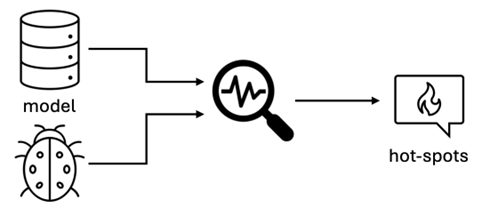
\includegraphics[width=0.5\textwidth]{3_identifying_gaps/benchmarking/profiling_methods/figures/profiling.png}
    \caption{Profiling methodology for a PRA tool.}
    \label{fig:profiling}
\end{figure}

For scram, profiling is performed on a model with 450 basic events for MOCUS MCUB, MOCUS REA, and ZBDD, and on a model with 350 basic events for BDD. For SAPHSOLVE, profiling is conducted on a model with 310 basic events, with truncation sizes varied to assess performance under different conditions. The SAPHSOLVE profiling is performed on a Windows 10 system due to observed differences in performance between the Linux and Windows versions.

\section{Benchmarking Results and Discussion}
The quick diagnostics phase evaluates the performance of scram and SAPHSOLVE across the generated synthetic models. Table~\ref{tab:quantified_input_files} summarizes the number of input files successfully quantified (out of 99 input files) by each engine and approach.

\begin{longtable}{@{}lccccc@{}}
\caption{Number of input files quantified by each engine and approach.}
\label{tab:quantified_input_files}\\
\toprule
\textbf{Approach} & \textbf{SCRAM} & \textbf{SCRAM} & \textbf{SCRAM} & \textbf{SCRAM} & \textbf{SAPHSOLVE} \\
 & \textbf{MOCUS-} & \textbf{MOCUS-} & \textbf{BDD} & \textbf{ZBDD-} & \textbf{MOCUS-} \\
 & \textbf{MCUB} & \textbf{REA} & & \textbf{REA} & \textbf{MCUB} \\
\midrule
\endfirsthead
\toprule
\textbf{Approach} & \textbf{SCRAM} & \textbf{SCRAM} & \textbf{SCRAM} & \textbf{SCRAM} & \textbf{SAPHSOLVE} \\
 & \textbf{MOCUS-} & \textbf{MOCUS-} & \textbf{BDD} & \textbf{ZBDD-} & \textbf{MOCUS-} \\
 & \textbf{MCUB} & \textbf{REA} & & \textbf{REA} & \textbf{MCUB} \\
\midrule
\endhead
\midrule
\endfoot
\bottomrule
\endlastfoot
Quantified files & 89 & 89 & 3 & 90 & 82 \\
\end{longtable}

The results indicate that the MOCUS and ZBDD algorithms in scram, as well as the MOCUS algorithm in SAPHSOLVE, are able to quantify the majority of models. The BDD approach in scram is limited by high memory requirements, resulting in only three successful quantifications. Models that cannot be quantified typically fail during the cut set generation step. For example, the ft-1300 model requires adjustment of the limit order in the size of minimal cut sets (MCS) to complete quantification. The relationship between the limit order and quantification time is exponential, as illustrated in Figure~\ref{fig:ft_1300}.

\begin{figure}[h!]
    \centering
    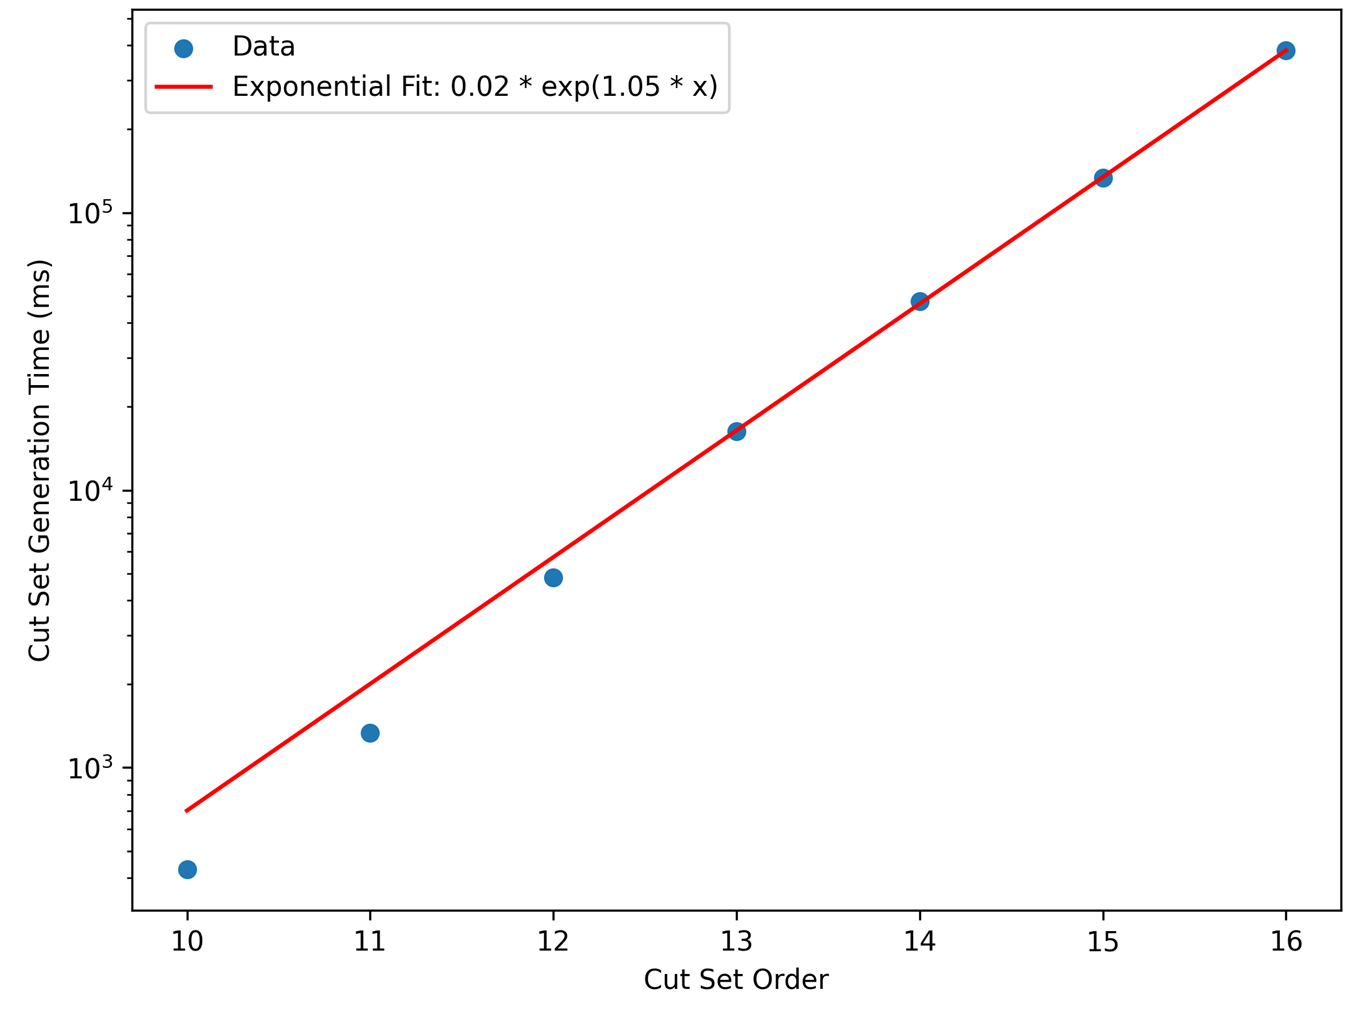
\includegraphics[width=0.75\textwidth]{3_identifying_gaps/benchmarking/profiling_methods/figures/ft_1300.png}
    \caption{Effect of limit order on MCS of scram for ft-1300 model.}
    \label{fig:ft_1300}
\end{figure}

A comparison of the number of cut sets generated by scram and SAPHSOLVE reveals that, in most cases, the results are consistent. However, differences are observed in a few models, particularly when using the ZBDD approach in scram. The probability results obtained by scram-MOCUS-MCUB and SAPHSOLVE-MOCUS-MCUB are identical, providing a valuable cross-check between the two engines.

The quantification time for scram is approximately linear with respect to the number of cut sets generated, as shown in Figure~\ref{fig:scram_quant_time}. While most models are quantified within the time limit, some require up to 20 minutes, which is not acceptable for practical PRA applications. The ZBDD approach is significantly faster than MOCUS, and BDD is the fastest when sufficient resources are available.

\begin{figure}[h!]
    \centering
    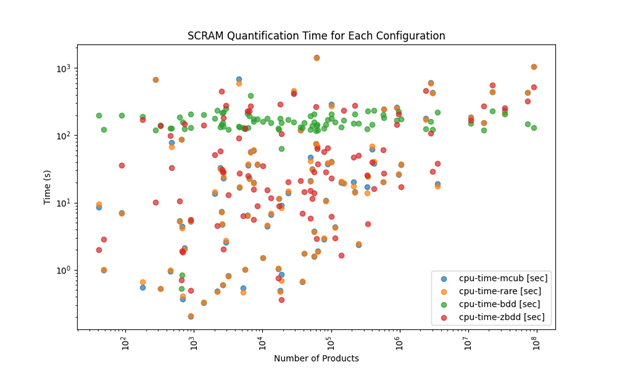
\includegraphics[width=0.9\textwidth]{3_identifying_gaps/benchmarking/profiling_methods/figures/scram_quant_time.png}
    \caption{scram quantification time results for all approaches.}
    \label{fig:scram_quant_time}
\end{figure}

Memory usage in scram increases with model size, as depicted in Figure~\ref{fig:scram_memory_usage}. BDD runs are generally infeasible due to excessive memory demands. The flat line in the figure represents the predefined memory limit.

\begin{figure}[H]
    \centering
    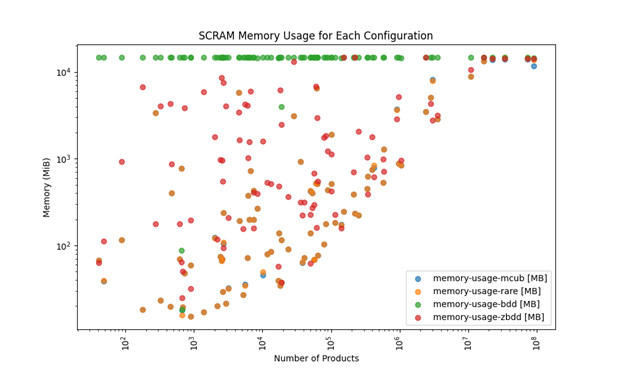
\includegraphics[width=0.9\textwidth]{3_identifying_gaps/benchmarking/profiling_methods/figures/scram_memory_usage.png}
    \caption{scram memory usage for all approaches.}
    \label{fig:scram_memory_usage}
\end{figure}

SAPHSOLVE quantifies 82 out of 99 models using the MOCUS approach with MCUB probability approximation. Its quantification time is consistently low, as shown in Figure~\ref{fig:saphsolve_quant_time}, due to early termination and efficient resource management. However, the Linux version of SAPHSOLVE is less capable than the Windows version when running without truncation.

\begin{figure}[H]
    \centering
    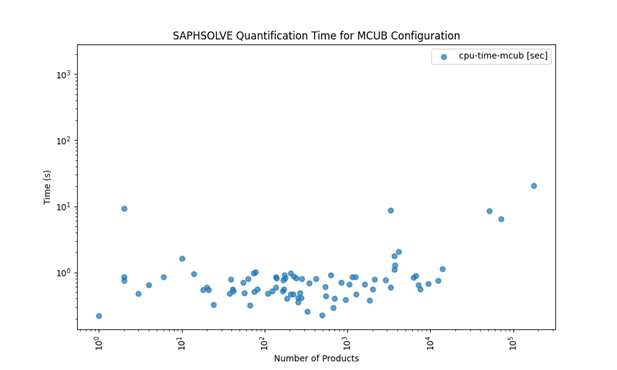
\includegraphics[width=0.9\textwidth]{3_identifying_gaps/benchmarking/profiling_methods/figures/saphsolve_quant_time.png}
    \caption{SAPHSOLVE quantification time results for MOCUS MCUB.}
    \label{fig:saphsolve_quant_time}
\end{figure}

SAPHOLVE's memory usage is also efficient, as depicted in Figure~\ref{fig:saphsolve_memory_usage}. The number of cut sets generated is slightly lower than in scram, which contributes to faster results.

\begin{figure}[H]
    \centering
    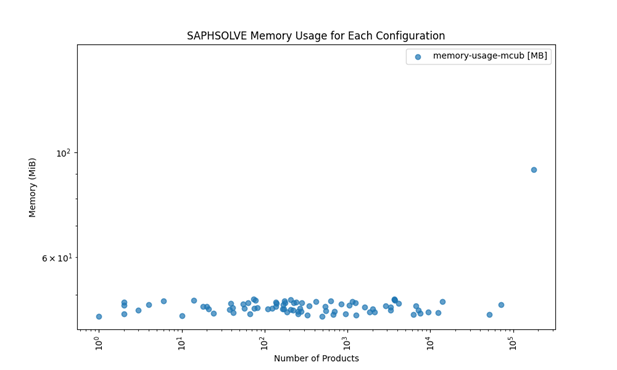
\includegraphics[width=0.9\textwidth]{3_identifying_gaps/benchmarking/profiling_methods/figures/saphsolve_memory_usage.png}
    \caption{SAPHSOLVE memory usage for MOCUS MCUB.}
    \label{fig:saphsolve_memory_usage}
\end{figure}

The benchmarking results highlight the trade-offs between speed, memory usage, and output detail. scram provides more detailed output but at the cost of higher resource consumption, while SAPHSOLVE is optimized for speed and minimal output.

\section{Profiling Results and Discussion}
Profiling provides detailed diagnostics of the quantification engines, enabling the identification of computational hotspots and inefficiencies. The profiling setup differs between scram and SAPHSOLVE due to differences in model formats, programming languages, and operating environments.

\subsection{scram Profiling}
Table~\ref{tab:scram_profiling} summarizes the profiling results for scram across different quantification approaches and input files.

\begin{table}[htbp]
    \centering
    \caption{Summary of profiling performance analysis results for scram.}
    \label{tab:scram_profiling}
    \begin{tabular}{|l|c|c|c|c|}
        \hline
        \textbf{Approach} & \textbf{MOCUS-} & \textbf{MOCUS-} & \textbf{BDD} & \textbf{ZBDD-} \\
        \textbf{-Approximation} & \textbf{MCUB} & \textbf{REA} & & \textbf{REA} \\
        \hline
        Input File & ft-450 & ft-450 & ft-350 & ft-450 \\
        Analysis Time [sec] & 431.230 & 426.177 & 62.566 & 320.072 \\
        Core Utilization & 0.972 out of 6 & -- & -- & -- \\
        \hline
    \end{tabular}
\end{table}

Hot spot analysis reveals that result reporting and cut set generation dominate computation time for the MOCUS and ZBDD algorithms. BDD construction is the primary bottleneck for the BDD approach. Figures~\ref{fig:vtune_scram_mocus_mcub} through~\ref{fig:vtune_scram_zbdd} provide VTune profiling results for each approach.

\begin{figure}[H]
    \centering
    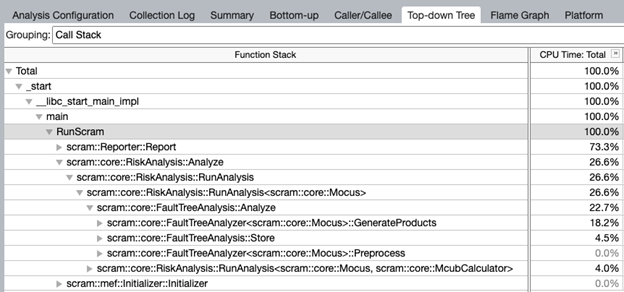
\includegraphics[width=0.9\textwidth]{3_identifying_gaps/benchmarking/profiling_methods/figures/vtune_scram_mocus_mcub.png}
    \caption{scram MOCUS MCUB VTune profiling results.}
    \label{fig:vtune_scram_mocus_mcub}
\end{figure}

\begin{figure}[H]
    \centering
    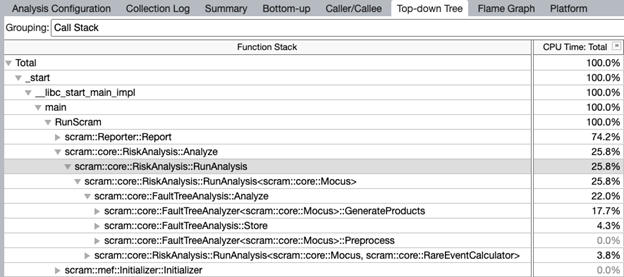
\includegraphics[width=0.9\textwidth]{3_identifying_gaps/benchmarking/profiling_methods/figures/vtune_scram_mocus_rea.png}
    \caption{scram MOCUS REA VTune profiling results.}
    \label{fig:vtune_scram_mocus_rea}
\end{figure}

\begin{figure}[H]
    \centering
    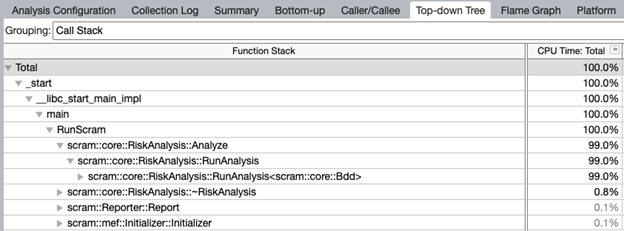
\includegraphics[width=0.9\textwidth]{3_identifying_gaps/benchmarking/profiling_methods/figures/vtune_scram_bdd.png}
    \caption{scram BDD VTune profiling results.}
    \label{fig:vtune_scram_bdd}
\end{figure}

\begin{figure}[H]
    \centering
    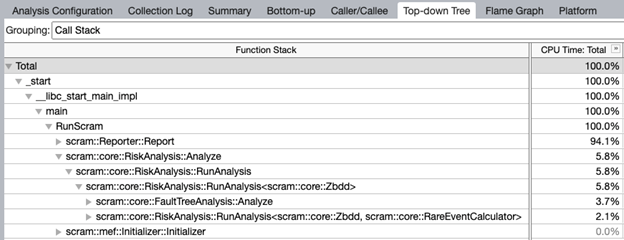
\includegraphics[width=0.9\textwidth]{3_identifying_gaps/benchmarking/profiling_methods/figures/vtune_scram_zbdd.png}
    \caption{scram ZBDD REA VTune profiling results.}
    \label{fig:vtune_scram_zbdd}
\end{figure}

\subsection{SAPHSOLVE Profiling}
Table~\ref{tab:saphsolve_profiling} presents the profiling results for SAPHSOLVE at different truncation sizes.

\begin{table}[htbp]
    \centering
    \caption{Summary of profiling performance analysis results for SAPHSOLVE.}
    \label{tab:saphsolve_profiling}
    \begin{tabular}{|l|c|c|c|}
        \hline
        \textbf{Truncation Size} & 16 & 18 & 20 \\
        \hline
        Input File Configuration & ft-310 & ft-310 & ft-310 \\
        Analysis Elapsed Time [sec] & 361.010 & 4,142.099 & 64,365.847 \\
        Number of Cut Sets & 11,490 & 102,444 & 761,472 \\
        Probability & $1.3388 \times 10^{-11}$ & -- & -- \\
        Physical Core Utilization & 1.306 out of 4 & -- & -- \\
        \hline
    \end{tabular}
\end{table}

The relationship between truncation size and calculation time in SAPHSOLVE is exponential, as shown in Figure~\ref{fig:saphsolve_truncation_time}. For large truncation sizes, performance degrades significantly, indicating a need for optimization in the size truncation implementation.

\begin{figure}[H]
    \centering
    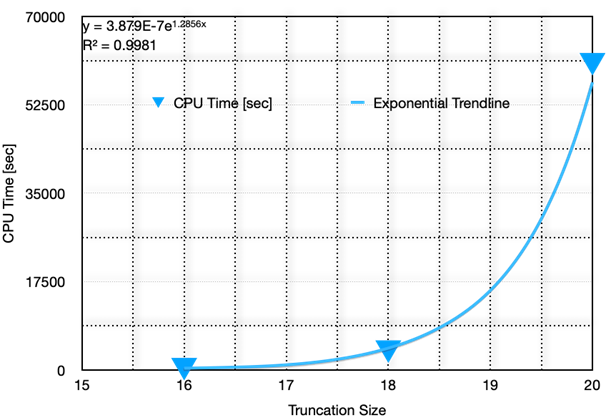
\includegraphics[width=0.8\textwidth]{3_identifying_gaps/benchmarking/profiling_methods/figures/saphsolve_truncation_time.png}
    \caption{SAPHSOLVE quantification time for different truncation sizes.}
    \label{fig:saphsolve_truncation_time}
\end{figure}

Table~\ref{tab:saphsolve_vtune} summarizes the VTune profiling results for SAPHSOLVE, highlighting the dominant functions and their contribution to total runtime.

\begin{table}[htbp]
    \centering
    \caption{SAPHSOLVE MOCUS MCUB VTune profiling results.}
    \label{tab:saphsolve_vtune}
    \begin{tabular}{|c|c|c|c|}
        \hline
        \textbf{Truncation Size} & \textbf{Function} & \textbf{CPU Time [sec]} & \textbf{Percentage Contribution [\%]} \\
        \hline
        16 & A & 175.643 & 49.5 \\
           & B & 52.284 & 14.7 \\
        18 & B & 1648.13 & 43 \\
           & A & 708.83 & 18.5 \\
        20 & B & 43893.54 & 72.2 \\
           & C & 3929.234 & 6.5 \\
           & A & 3580.815 & 5.9 \\
        \hline
    \end{tabular}
\end{table}

Functions responsible for cut set generation dominate the runtime, especially as truncation size increases. This observation underscores the importance of efficient cut set management in large scale PRA quantification.

\section{Conclusion}
Benchmarking and profiling are indispensable for the rigorous evaluation and improvement of PRA quantification engines. The results presented in this chapter demonstrate that while both scram and SAPHSOLVE are capable of quantifying large synthetic models, their performance characteristics differ significantly. scram offers detailed output and multiple quantification approaches but at the cost of higher resource consumption. SAPHSOLVE is optimized for speed and minimal output but exhibits performance degradation for large truncation sizes. Profiling reveals that cut set generation is the primary computational bottleneck in both engines. These insights provide a foundation for targeted optimization and future development of high performance PRA tools.

\chapter{Task IV: Application to Multi-Hazard PRA Models}
\label{cha:task_iv}

\section{Generic PWR Model with Multi-Hazard Capabilities}
\label{sec:PWR_model}
A generic \acrshort{pwr} model was extended from a single-hazard configuration~\cite{Smith2021Generic} to incorporate hazard interactions.  The workflow comprises two sequential stages:

\begin{enumerate}
  \item \textbf{Model construction} with an in-house tool, OpenMHA~\cite{Batikh2024OpenMHA}, resulting in an updated \acrshort{mar-d} file containing combined fault-tree/event-tree logic and failure data.
  \item \textbf{Model quantification} with SAPHIRE 8, performed either via the \acrshort{gui} or the \acrshort{dll}-based \acrshort{saphsolve} engine.
\end{enumerate}

\subsection{Model Building with OpenMHA}
OpenMHA is a scenario-based framework that
\begin{itemize}
  \item stores layout, logic, and \acrshort{ssc} metadata in a MongoDB instance;
  \item provides hazard-specific classes (\texttt{Fire}, \texttt{Flooding}, \texttt{Seismic}, \texttt{Tsunami}) that assemble fault-tree logic and call external physics simulators; and
  \item exports a fully populated \acrshort{mar-d} file for downstream solvers.
\end{itemize}
The present study focuses on the \texttt{Seismic} class, which explicitly models main shocks and correlated aftershocks.

\subsection{Model Quantification with SAPHIRE}
\label{sec:saphire_quant}
The \acrshort{mar-d} file is imported into SAPHIRE, followed by compilation of a linkage-rule file. Algorithm~\ref{alg:saphire_aftershock_linkage} shows an excerpt that assigns aftershock-dependent flags. Algorithm~\ref{alg:saphsolve_autoquantification} details automated invocation of the \acrshort{dll} solver. Probability truncation is applied at user-defined thresholds $P_{\text{cut}} \;=\;10^{-k}$, where $k\in\{7,20\}$ in this study.

%----------- Linkage rules ---------------------------------------
\begin{algorithm}[h!]
\caption{Excerpt of SAPHIRE linkage rules for the aftershock model}
\label{alg:saphire_aftershock_linkage}
\begin{algorithmic}[1]
\If{SLOCA\_EQ1\_FT \textbf{and} LOOP\_EQ1\_FT}
  \State EVENTREE(EQK\_BIN1) $\gets$ FLAG(ETF\_EQ1\_SL)
\ElsIf{LLOCA\_EQ1\_FT \textbf{and} LOOP\_EQ1\_FT}
  \State EVENTREE(EQK\_BIN1) $\gets$ FLAG(ETF\_EQ1\_LL)
\Else
  \State EVENTREE(EQK\_BIN1) $\gets$ FLAG(ETF\_EQ1)
\EndIf
\If{INIT(IE\_EQ\_BIN1)}
  \State EVENTREE(EQK\_BIN1) $\gets$ ENDSTATE(CD\_EQ)
  \State EVENTREE(EQK\_BIN1) $\gets$ FLAG(T\_1)
\EndIf
\end{algorithmic}
\end{algorithm}

%----------- Pseudocode listing ----------------------------------
\begin{algorithm}[h!]
\caption{High-level pseudocode for automated quantification via \acrshort{saphsolve}}
\label{alg:saphsolve_autoquantification}
\begin{algorithmic}[1]
\State \textbf{import} \texttt{os, threading, ctypes, time}
\State Load \texttt{solve.dll}; \textbf{exit} on failure
\Function{SolveJSON}{$\textit{inFile},\,\textit{outDir}$}
  \State Generate \textit{outFile}$\leftarrow$replaceExt(\textit{inFile},.JSCut)
  \State \textit{t}$\gets$time.solveDLL(\textit{inFile})
  \State \textbf{handle} exceptions
\EndFunction
\Function{SolveThread}{$\textit{files},\,\textit{inDir},\,\textit{outDir}$}
  \ForAll{\textit{f} $\in$ \textit{files}} \Call{SolveJSON}{\textit{f}} \EndFor
\EndFunction
\Function{Main}{}
  \State Enumerate *.JSInp files; build \textit{chunks} per CPU core
  \State Serial timing $\gets$ \Call{SolveJSON}{\textit{each file}}
  \State Parallel timing $\gets$ \textbf{spawn} \Call{SolveThread}{\dots}
\EndFunction
\end{algorithmic}
\end{algorithm}

\subsection{Quantification Results and Discussion}

%----------- Results table ---------------------------------------
\begin{table}[h!]
\centering
\caption{Solve time for the generic \acrshort{pwr} aftershock model at two truncation levels.}
\label{tab:solve_time_generic_pwr}
\begin{tabular}{@{}lS[table-format=3.0]S[table-format=5.2]@{}}
\toprule
\textbf{Input / $P_{\text{cut}}$} & 
\multicolumn{1}{c}{\textbf{\acrshort{gui} [s]}} & 
\multicolumn{1}{c}{\textbf{\acrshort{dll} [s]}} \\
\midrule
EQK\_BIN1 / $10^{-7}$  & 643  & 14.97 \\
EQK\_BIN1 / $10^{-20}$ & {---} & 11784.49 \\
\bottomrule
\end{tabular}
\end{table}

The \acrshort{gui} requires extensive pre-processing, whereas the direct \acrshort{dll} invocation eliminates that overhead for already-generated JSON inputs (Table~\ref{tab:solve_time_generic_pwr}).  At $P_{\text{cut}}=10^{-20}$ the \acrshort{gui} timed out, yet the \acrshort{dll} solution completed in \SI{3.3}{h}.  This highlights the importance of optimizing pre-processing routines for users who rely solely on the graphical interface.

Comparing the count and values of \acrfull{mcs} for $k=7$ and $k=20$, as shown in Table~\ref{tab:PWR-aftershock-trunc}, we observe a significant increase in the number of \acrshort{mcs} with the finer truncation value, as expected. However, discrepancies in probability results were also observed. In some cases, these discrepancies are unacceptably high.

\sisetup{ 
  scientific-notation = true,
  table-format        = 1.2e-2,
  round-mode          = places,
  round-direction     = up,
  round-precision     = 2,
  group-separator     = {,},
  group-minimum-digits= 4,
  table-number-alignment = center,
}
\begin{longtable}{@{}lrrrSSS@{}}
\caption{Quantification results for the \acrshort{pwr} aftershock model at two truncation levels.}
\label{tab:PWR-aftershock-trunc}\\
\toprule
\multirow{2}{*}{\textbf{Input}} &
  \multicolumn{1}{l}{\multirow{2}{*}{\textbf{\begin{tabular}[c]{@{}l@{}}Sequence\\ Count\end{tabular}}}} &
  \multicolumn{2}{c}{\textbf{\# Minimal Cut Sets}} &
  \multicolumn{2}{c}{\textbf{Probability}} &
  \multicolumn{1}{c}{\multirow{2}{*}{\textbf{\begin{tabular}[c]{@{}l@{}}Percentage\\ Difference\end{tabular}}}} \\* \cmidrule(lr){3-6}
 &
  \multicolumn{1}{l}{} &
  \multicolumn{1}{l}{$P_{\text{cut}} = 10^{-7}$} &
  \multicolumn{1}{l}{$P_{\text{cut}} = 10^{-20}$} &
  \multicolumn{1}{l}{$P_{\text{cut}} = 10^{-7}$} &
  \multicolumn{1}{l}{$P_{\text{cut}} = 10^{-20}$} &
  \multicolumn{1}{l}{} \\* \midrule
\endhead
%
\bottomrule
\endfoot
%
\endlastfoot
%
\textbf{1} & 30 & 668 & 31,132,273 & 3.1090E-03 & 3.1656E-03 & 1.79\%  \\
\textbf{2} & 3  & 47  & 17,938     & 2.8278E-05 & 3.0606E-05 & 7.61\%  \\
\textbf{3} & 3  & 42  & 144,013    & 1.4515E-04 & 1.4668E-04 & 1.04\%  \\
\textbf{4} & 8  & 11  & 580,190    & 4.4697E-06 & 7.3165E-06 & 38.91\% \\
\textbf{5} & 8  & 29  & 1,314,498  & 2.8961E-05 & 3.1139E-05 & 6.99\%  \\
\textbf{6} & 33 & 868 & 21,248,913 & 2.6158E-03 & 2.8147E-03 & 7.07\%  \\* \bottomrule
\end{longtable}

\section{Benchmarked Metrics}
\section{Available Tools - Versions \& Descriptions}

\chapter{Optimizing Available Tools}
 % \sectionP{}
point to papers and egemen's dissertation

 \subsection{Instrumenting for Profiling}
 \section{Profiling Metrics}
 \subsection{CPU Usage, Memory Footprint, Parallel Scalability}
 \subsection{Real-Time vs. Offline Calculation Needs}
 \subsection{Identifying Kernel Hotspots and Bottlenecks}
\section{Picking Low Hanging Fruit - Optimizations}